\documentclass[../notes.tex]{subfiles}

\pagestyle{main}
\renewcommand{\chaptermark}[1]{\markboth{\chaptername\ \thechapter\ (#1)}{}}
\setcounter{chapter}{4}

\begin{document}




\chapter{Non-Inertial Reference Frames}
\section{Rotating Reference Frames}
\begin{itemize}
    \item \marginnote{10/23:}Recap: Scattering.
    \begin{itemize}
        \item For a particular central force, we can find $b(\Theta)$.
        \item The differential cross-section (what is this??).
        \item For a general potential $V(r)$, we can use the orbit equation to solve for the angular change from $r_\text{min}$ to $r_\text{max}$ and back.
        \begin{itemize}
            \item The "and back" part is why we get the 2 coefficient!
            \item HW: Use this to derive a general relationship $b(\Theta)$ for any $V$.
        \end{itemize}
        \item For a \textbf{closed}, non-circular orbit, we must have integers $a,b$ such that
        \begin{equation*}
            2\pi = \Delta\theta\cdot\frac{a}{b}
        \end{equation*}
        \begin{itemize}
            \item Curiously, for $V(r)=kr^{n+1}$, only $n=1$ (attractive harmonic oscillator) and $n=-2$ (inverse square law) have this property!
            \item Does she mean $n=-1$ if we're talking about inverse square law \emph{potential}?? Also, need for what??
        \end{itemize}
    \end{itemize}
    \item Today.
    \begin{itemize}
        \item Rotating reference frames.
        \item Gravity + Coriolis Effect.
    \end{itemize}
    \item \textbf{Vector angular velocity}: The vector defined as follows, which describes the angular velocity of a rotating body. \emph{Denoted by} $\bm{\vec{\omega}}$. \emph{Given by}
    \begin{equation*}
        \vec{\omega} = \omega\khat
    \end{equation*}
    \item Example:
    \begin{equation*}
        \omega_\text{earth} = \frac{2\pi}{\SI{24}{\hour}}
        = \SI{7.3e-5}{\per\second}
    \end{equation*}
    \item Define vectors $\ihat,\jhat,\khat$ that \emph{rotate} about $\khat$ to remain fixed on the surface of the rotating body.
    \item For a fixed vector $\hat{r}$ on a rotating body, the change in $\vec{r}$ with respect to time according to an inertial observer is given by
    \begin{equation*}
        \dv{\vec{r}}{t} = \vec{v}
        = \vec{\omega}\times\vec{r}
    \end{equation*}
    \begin{figure}[h!]
        \centering
        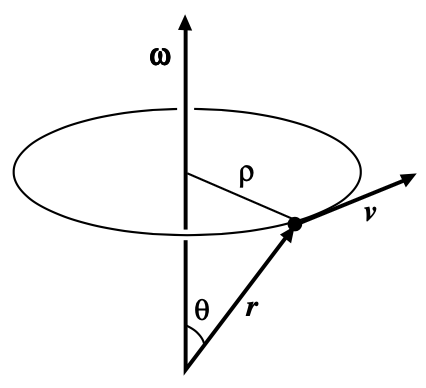
\includegraphics[width=0.25\linewidth]{../ExtFiles/Vrotation.png}
        \caption{Rotational velocity.}
        \label{fig:Vrotation}
    \end{figure}
    \begin{itemize}
        \item Proof: $v=\omega\rho=r\omega\sin\theta$.
    \end{itemize}
    \item The specific case where $\vec{r}=\ihat,\jhat,\khat$.
    \begin{align*}
        \dv{\ihat}{t} &= \vec{\omega}\times\ihat&
        \dv{\jhat}{t} &= \vec{\omega}\times\jhat&
        \dv{\khat}{t} &= \vec{\omega}\times\khat
    \end{align*}
    \item The case where the vector is time-dependent.
    \begin{itemize}
        \item Let $\vec{b}=b_x\ihat+b_y\jhat+b_z\khat$, where $b_x,b_y,b_z$ are functions of time.
        \item Define notions of \textbf{absolute} and \textbf{relative} velocity.
        \item Relationship between the above two quantities:
        \begin{align*}
            \dv{\vec{b}}{t} &= (\dot{b}_x\ihat+\dot{b}_y\jhat+\dot{b}_z\khat)+\left( b_x\dv{\ihat}{t}+b_y\dv{\jhat}{t}+b_z\dv{\khat}{t} \right)\\
            &= \dot{\vec{b}}+b_x\vec{\omega}\times\ihat+b_y\vec{\omega}\times\jhat+b_z\vec{\omega}\times\khat\\
            &= \dot{\vec{b}}+\vec{\omega}\times\vec{b}
        \end{align*}
        \item The last line above is definitely worth remembering.
    \end{itemize}
    \item \textbf{Absolute} (velocity): The time rate of change of $\vec{r}$ as observed in an \emph{inertial} frame. \emph{Denoted by} $\bm{\textbf{d}\vec{r}/\textbf{d}t}$, $\bm{\vec{v}_\textbf{inertial observer}}$, $\bm{\vec{v}}$. \emph{Given by}
    \begin{equation*}
        \dv{\vec{r}}{t} = \dot{\vec{r}}+\vec{\omega}\times\vec{r}
    \end{equation*}
    \item \textbf{Relative} (velocity): The time rate of change of $\vec{r}$ as observed in a \emph{rotating} frame. \emph{Denoted by} $\bm{\dot{\vec{r}}}$. \emph{Given by}
    \begin{equation*}
        \dot{\vec{r}} = \dot{r}_x\ihat+\dot{r}_y\jhat+\dot{r}_z\khat
    \end{equation*}
    \item \textbf{Absolute} (acceleration): The time rate of change of $\vec{v}_\text{inertial observer}$ as observed in an \emph{inertial} frame. \emph{Denoted by} $\bm{\textbf{d}\vec{v}/\textbf{d}t}$, $\bm{\vec{a}_\textbf{inertial observer}}$, $\bm{\textbf{d}^2\vec{r}/\textbf{d}t^2}$. \emph{Given by}
    \begin{equation*}
        \dv{\vec{v}}{t} = \dot{\vec{v}}+\vec{\omega}\times\vec{v}
    \end{equation*}
    \item \textbf{Relative} (acceleration): The time rate of change of $\vec{v}_\text{inertial observer}$ as observed in a \emph{rotating} frame. \emph{Denoted by} $\bm{\dot{\vec{v}}}$. \emph{Given by}
    \begin{equation*}
        \dot{\vec{v}} = \ddot{\vec{r}}+\vec{\omega}\times\dot{\vec{r}}
    \end{equation*}
    \begin{itemize}
        \item Note that this result only holds when $\vec{\omega}$ is constant.
    \end{itemize}
    \item Let's investigate the $\vec{\omega}\times\vec{v}$ from the definition of absolute acceleration a bit more closely.
    \begin{itemize}
        \item Substituting in the definition of $\vec{v}$ as $\dot{\vec{r}}+\vec{\omega}\times\vec{r}$, we obtain
        \begin{equation*}
            \vec{\omega}\times\vec{v} = \vec{\omega}\times\dot{\vec{r}}+\vec{\omega}\times(\vec{\omega}\times\vec{r})
        \end{equation*}
        \item Thus, we can alternatively write an expression for absolute acceleration as follows.
        \begin{equation*}
            \dv[2]{\vec{r}}{t} = \ddot{\vec{r}}+2\vec{\omega}\times\dot{\vec{r}}+\vec{\omega}\times(\vec{\omega}\times\vec{r})
        \end{equation*}
        \item This last term points toward the axis of rotation.
        \begin{itemize}
            \item See \textcite{bib:KibbleBerkshire}, Q5.19, for more.
        \end{itemize}
    \end{itemize}
    \item Using the above discussion and result, we will analyze physics near Earth's surface.
    \begin{itemize}
        \item For a particle moving under gravity $m\vec{g}=-GMm/R^2\approx 9.81m$ and under other, additional forces $\vec{F}$, the equation of motion is
        \begin{equation*}
            m\vec{a}_\text{inertial} = m\vec{g}+\vec{F}
        \end{equation*}
        \item What we measure on earth is $m\ddot{\vec{r}}$. It is related to the above quantities via the result from the previous discussion as follows.
        \begin{equation*}
            m\ddot{\vec{r}} = m\vec{g}+\vec{F}-2m\vec{\omega}\times\dot{\vec{r}}-m\vec{\omega}\times(\vec{\omega}\times\vec{r})
        \end{equation*}
        \begin{itemize}
            \item Note that the $-2m\vec{\omega}\times\dot{\vec{r}}$ and $-m\vec{\omega}\times(\vec{\omega}\times\vec{r})$ terms are known as the \textbf{Coriolis} and \textbf{centrifugal} forces, respectively.
            \item These forces are "apparent" or "fictitious" forces caused by our rotational motion; they are not \emph{actual} forces like pushing on something.
        \end{itemize}
    \end{itemize}
    \item Consider a particle that is not under the influence of any force besides gravity (e.g., a projectile).
    \begin{itemize}
        \item Suppose it lies at latitude $\pi/2-\theta$ and longitude $\phi$.
        \item Refresher: On Earth, $\vec{\omega}=\omega\khat$.
        \item There are three local coordinates on Earth's surface: \textbf{East} ($\hat{e}$), \textbf{north} ($\hat{n}$), and \textbf{up} ($\hat{r}$).
        \begin{itemize}
            \item Note that naturally, up shares a symbol with the radial vector because they both point in the same direction: Away from the center of the Earth/spherical body in question.
        \end{itemize}
        \item Note: From trigonometry,
        \begin{equation*}
            \vec{\omega} = \omega\cos\theta\hat{r}+\omega\sin\theta\hat{n}
        \end{equation*}
        \begin{itemize}
            \item It follows that the $\hat{r}$ component of $\vec{\omega}$ is inwards in the southern hemisphere!
        \end{itemize}
        \item Thus, in terms of all of these local coordinates, the relative acceleration of the particle can be described as follows.
        \begin{equation*}
            \ddot{\vec{r}} = -g\hat{r}-2\omega(\cos\theta\hat{r}+\sin\theta\hat{n})\times(\dot{r}_r\hat{r}+\dot{r}_e\hat{e}+\dot{r}_n\hat{n})-\omega^2R\sin\theta(-\sin\theta\hat{r}+\cos\theta\hat{n})
        \end{equation*}
        \begin{itemize}
            \item Note that the last term comes from expanding $(\omega\cos\theta\hat{r}+\omega\sin\theta\hat{n})\times[(\omega\cos\theta\hat{r}+\omega\sin\theta\hat{n})\times R\hat{r}]$. We take $\vec{r}=R\hat{r}$ here because we are using polar coordinates, not $\ihat,\jhat,\khat$.
        \end{itemize}
        \item Using the $\hat{r}$ component of the above, we can reconstruct the gravitational force at Earth's surface.
        \begin{equation*}
            \ddot{r}_r = -g+2\omega\sin\theta\dot{r}_e+\omega^2R\sin^2\theta
            \approx -g
        \end{equation*}
        \begin{itemize}
            \item We say that the sum of the three terms above is approximately equal to the first term because the first term is 2-5 orders of magnitude larger than the other two ($\omega=\SI{7.3e-5}{\per\second}$ and $\omega^2R=\SI[per-mode=symbol]{34}{\milli\meter\per\second\squared}$).
        \end{itemize}
        \item Similarly, the other two components are
        \begin{align*}
            \ddot{r}_n &= -2\omega\cos\theta\dot{r}_e-\omega^2R\sin\theta\cos\theta&
            \ddot{r}_e &= 2\omega\cos\theta\dot{r}_n-2\omega\sin\theta\dot{r}_r
        \end{align*}
    \end{itemize}
    \item Measuring $\vec{g}$.
    \begin{itemize}
        \item Because the earth is rotating, we must necessarily measure the apparent gravity $\ddot{r}_r$ and then mathematically manipulate our data to get the true answer.
        \item Note, however, that in such an experiment, the experimental setup is generally stationary. Thus, with $\dot{r}=0$, $\dot{r}_e=0$, so we may discount the Coriolis force.
        \item In particular, this means that
        \begin{equation*}
            \vec{g}_\text{apparent} = \vec{g}-\vec{\omega}\times(\vec{\omega}\times\vec{r})
            = (-g+\omega^2R\sin^2\theta)\hat{r}-(\omega^2R\sin\theta\cos\theta)\hat{n}
        \end{equation*}
        \item Define the angle between the true and apparent verticals to be
        \begin{equation*}
            \alpha \approx \sin^{-1}\left( \frac{\omega^2R\sin\theta\cos\theta}{1-g+\omega^2R\sin^2\theta} \right)
            \approx \frac{\omega^2R}{g}\sin\theta\cos\theta
        \end{equation*}
        \begin{itemize}
            \item Where does the 1 in the denominator come from?? Why sine, not tangent? How are you doing the simplification?
        \end{itemize}
        \item By the above definition, $\alpha$ maxes out when $\theta=\ang{45}$, at about \ang{60}$6'$.
        \item Additionally, at the poles ($\theta=0,\pi$), $\alpha=0$ and $g_\text{apparent}=g$.
        \begin{itemize}
            \item At the equator, $g_\text{apparent}=g-\omega^2R$ is at its minimum.
        \end{itemize}
        \item Note that (not accounting for the Earth being oblong), we have that
        \begin{equation*}
            \Delta g = g-g_\text{apparent} = \SI[per-mode=symbol]{34}{\milli\meter\per\second}
        \end{equation*}
    \end{itemize}
    \item The Coriolis force.
    \begin{itemize}
        \item The acceleration due to the Coriolis force is as follows.
        \begin{align*}
            \ddot{r}_r &\approx -g+2\omega\sin\theta\dot{r}_e&
            \ddot{r}_n &\approx -2\omega\cos\theta\dot{r}_e&
            \ddot{r}_e &\approx 2\omega\cos\theta\dot{r}_n-2\omega\sin\theta\dot{r}_r
        \end{align*}
        \begin{itemize}
            \item Note that we say "approximately equal" for now because, as mentioned above, there are some parameters we're not yet accounting for, such as the Earth being oblong.
            \item Why is $-g$ included in $\ddot{r}_r$??
        \end{itemize}
        \item Examples.
        \begin{enumerate}
            \item Drop something straight down.
            \begin{itemize}
                \item When something is dropped straight down, it has a negative radial velocity, i.e., $\dot{r}_r<0$.
                \item It follows by the above that $\ddot{r}_e>0$, so the particle lands slightly east because the Earth has rotated westward under it!
                \item Note: Technically, this acceleration in the east direction induces an acceleration in the north direction which, in turn, modifies the acceleration in the east direction. However, we can neglect these terms because they are second order in $\omega$.
            \end{itemize}
            \item Horizontal flow.
            \begin{itemize}
                \item Think trade winds, cyclones.
                \item It is the Coriolis effect that makes it so that in the northern hemisphere, storms rotate clockwise, while in the southern hemisphere, they rotate counterclockwise.
            \end{itemize}
        \end{enumerate}
    \end{itemize}
\end{itemize}



\section{Office Hours (Jerison)}
\begin{itemize}
    \item The convenient choice for the zero of energy is the energy of the particle when it's at $\infty$.
    \item $E,k$ are independent; it is possible to have a hyperbolic orbit with \emph{deflection} and with \emph{attraction}.
    \begin{itemize}
        \item The sign of $k$ corresponds to \emph{which branch} of the hyperbola you're on, i.e., are you orbiting the focus (attractive) or coming within a certain distance of it and then flying away!
        \item In the $e=0$ case, we can \emph{only} have attractive motion, however!
        \item In the case of an attractive force, we can have a circular, elliptical, parabolic, or hyperbolic orbit. In the case of a repulsive force, we can only have a hyperbolic orbit.
    \end{itemize}
\end{itemize}



\section{Coriolis Effect and Larmor Effect}
\begin{itemize}
    \item \marginnote{10/25:}Recap.
    \begin{itemize}
        \item Rotating reference frames and motion near Earth.
        \item For a rotating body, we define three vectors that rotate with it: $\ihat,\jhat,\khat$.
        \item $\vec{\omega}=\omega\khat$ is chosen parallel to $\khat$ along the rotation axis.
        \item If we have a vector $\vec{b}$ moving along the surface of the rotating body, then
        \begin{equation*}
            \dv{\vec{b}}{t} = \dot{\vec{b}}+\vec{\omega}\times\vec{b}
        \end{equation*}
        \begin{itemize}
            \item If $\dv*{\vec{b}}{t}=\vec{\omega}\times\vec{b}$ for some $\vec{b}$, then $\vec{b}$ is constant in magnitude and rotating about the axis defined by $\vec{\omega}$ at rate $\omega$.
        \end{itemize}
        \item Rotating frames have new equations of motion:
        \begin{equation*}
            m\ddot{\vec{r}} = m\dv[2]{\vec{r}}{t}-2m\vec{\omega}\times\dot{\vec{r}}-m\vec{\omega}\times(\vec{\omega}\times\vec{r})
        \end{equation*}
        \item Near earth, we measure
        \begin{equation*}
            m\ddot{\vec{r}} = m\vec{g}+\vec{F}\underbrace{-2m\vec{\omega}\times\dot{\vec{r}}\vphantom{()}}_\text{Coriolis}\underbrace{-m\vec{\omega}\times(\vec{\omega}\times\vec{r})}_\text{centrifugal}
        \end{equation*}
        \item Effects.
        \begin{enumerate}
            \item Centrifugal force: Points outwards from the axis of motion, inducing a very small ($\sim 0.3\%$) correction to gravity called \emph{apparent gravity}.
            \item Coriolis force: An adjustment by
            \begin{equation*}
                -2m\vec{\omega}\times\dot{\vec{r}} = 2m\omega(\underbrace{\dot{\vec{r}}_n\cos\theta-\dot{\vec{r}}_r\sin\theta}_{\hat{e}},\underbrace{-\dot{\vec{r}}_e\cos\theta}_{\hat{n}},\underbrace{\dot{\vec{r}}_e\sin\theta}_{\hat{r}})
            \end{equation*}
        \end{enumerate}
    \end{itemize}
    \item Example to visualize some of last time's content: (Fictional) Battle of Chicago.
    \begin{itemize}
        \item Aliens are attacking the Willis Tower! It is up to us to fire a cannon at them and destroy them! But how far will the Coriolis effect throw off our shot over such a distance?
        \item Initial conditions.
        \begin{itemize}
            \item We are approximately (we'll say exactly for the sake of the problem) \SI{11.4}{\kilo\meter} due south of the Willis tower.
            \item To ensure that the cannonball can make it to Willis Tower, we fire our cannon at \ang{45} with initial velocity $v=\SI[per-mode=symbol]{334}{\meter\per\second}$.
            \item Chicago's latitude can be described by $\theta_\text{Chicago}=\ang{48.2}$.
        \end{itemize}
        \item Defining variables.
        \begin{itemize}
            \item If $v=\SI[per-mode=symbol]{334}{\meter\per\second}$, then the northern and radial components $v_n=v_r=\SI[per-mode=symbol]{236}{\meter\per\second}$.
            \item The time of flight will be $\Delta t_\text{flight}=2v_r/g$.
            \begin{itemize}
                \item We won't need the actual value, but it is \SI{48.1}{\second}, if you're curious.
            \end{itemize}
            \item We approximate $\dot{\vec{r}}_n=v_{n,\text{init}}$. Note that this makes it so that the northern and radial components of the Coriolis force are of order $\omega^2$, i.e., negligible.
        \end{itemize}
        \item EOM.
        \begin{equation*}
            m\ddot{\vec{r}} = 2m\omega(v_n\cos\theta-v_r\sin\theta)\hat{e}-mg\hat{r}
        \end{equation*}
        \begin{itemize}
            \item In scalar form, the above vector equation becomes
            \begin{equation*}
                m
                \begin{bmatrix}
                    \ddot{r}_e\\
                    \ddot{r}_n\\
                    \ddot{r}_r\\
                \end{bmatrix}
                = m
                \begin{bmatrix}
                    2\omega(v_n\cos\theta-v_r\sin\theta)\\
                    0\\
                    -g\\
                \end{bmatrix}
            \end{equation*}
        \end{itemize}
        \item Since $\ddot{r}_r=-g$, integration gives $\dot{r}=v_r-gt$.
        \item Substituting this into the other equation, simplifying (including with $v_n=v_r$), and integrating with $r_e(0)=\dot{r}_e(0)=0$, we obtain
        \begin{align*}
            \ddot{r}_e &= 2\omega[v_r\cos\theta-(v_r-gt)\sin\theta]\\
            &= 2\omega[v_r(\cos\theta-\sin\theta)+gt\sin\theta]\\
            r_e &= 2\omega\left[ v_r(\cos\theta-\sin\theta)\frac{t^2}{2}+\frac{gt^3}{6}\sin\theta \right]
        \end{align*}
        \item Substituting in our expression for the time of flight, we obtain
        \begin{equation*}
            r_e = 2\omega\frac{v_r^3}{g^2}\left( 2\cos\theta_\text{Chicago}-\frac{2}{3}\sin\theta_\text{Chicago} \right)
        \end{equation*}
        \item Plugging in $\omega=\SI{7.29e-5}{\per\second}$, $v_r=\SI[per-mode=symbol]{236}{\meter\per\second}$, $g=\SI[per-mode=symbol]{9.81}{\meter\per\second}$, and $\theta_\text{Chicago}=\ang{48.2}$, we obtain the final answer
        \begin{equation*}
            r_e = \SI{16.7}{\meter}\,\hat{e}
        \end{equation*}
    \end{itemize}
    \item We now start in on some new content.
    \item Motion in a magnetic field.
    \begin{itemize}
        \item A particle of charge $q$ moving with velocity $\vec{v}$ in a constant magnetic field $\vec{B}$ experiences a force
        \begin{equation*}
            \vec{F} = q\vec{v}\times\vec{B}
        \end{equation*}
        \item It follows that
        \begin{align*}
            m\dv{\vec{v}}{t} &= q\vec{v}\times\vec{B}\\
            \dv{\vec{v}}{t} &= \underbrace{-\frac{q}{m}\vec{B}}_{\vec{\omega}}\times\vec{v}\\
        \end{align*}
        \item Implication: In a magnetic field, a charged particle's velocity vector rotates about $\vec{B}$ with frequency $\omega=qB/m$.
        \item Implication: $\vec{v}\parallel\vec{B}$ implies $\dv*{\vec{v}}{t}=0$.
        \item Implication: $\vec{v}\perp\vec{B}$ implies that $\vec{v}$ remains constant in magnitude but directionally rotates about $\vec{B}$.
        \begin{itemize}
            \item Example: $\vec{v}(t)=v\cos(\omega t)\hat{x}+v\sin(\omega t)\hat{y}$.
            \item Integrating the above yields an equation for circular motion about $(x_0,y_0+v/\omega)$ with radius $r=v/\omega$.
            \begin{equation*}
                \vec{r}(t) = \left( x_0+\frac{v}{\omega}\sin(\omega t) \right)\hat{x}+\left( y_0+\frac{v}{\omega}-\frac{v}{\omega}\cos(\omega t) \right)
            \end{equation*}
            \item Note that returning the definition of $\omega$, we obtain the following alternate expression for the radius of the motion.
            \begin{equation*}
                r = \frac{mv}{qB}
            \end{equation*}
        \end{itemize}
    \end{itemize}
    \item A quick note on cyclotrons.
    \begin{figure}[h!]
        \centering
        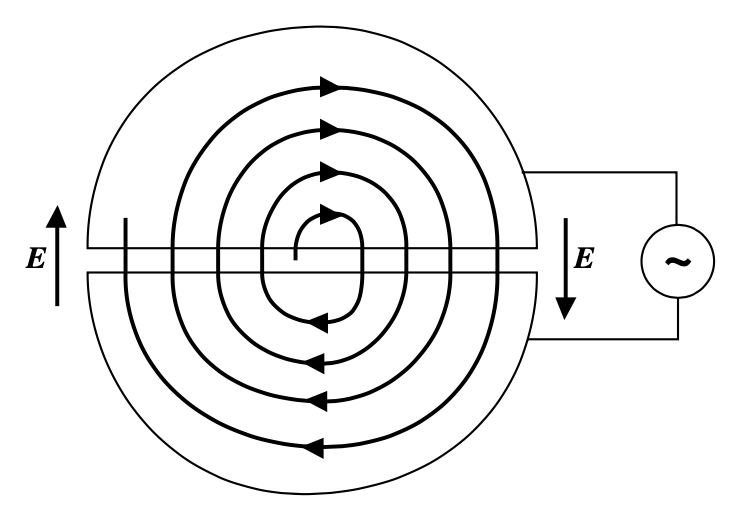
\includegraphics[width=0.35\linewidth]{../ExtFiles/cyclotron.png}
        \caption{A cyclotron.}
        \label{fig:cyclotron}
    \end{figure}
    \begin{itemize}
        \item Charged particles can be accelerated by using a strong magnetic field (perpendicular to the page) to constrain the particles to approximately circular motion, and then an alternating electric potential to accelerate them across a gap over and over again.
        \item To achieve maximum acceleration, the angular frequency of the alternating voltage is chosen to correspond to the \textbf{cyclotron frequency}. This is analogous to the resonance condition of the driven harmonic oscillator!
    \end{itemize}
    \item \textbf{Cyclotron frequency}: The angular frequency at which a charged particle with nonzero velocity rotates under a given cyclotron's magnetic field. \emph{Denoted by} $\bm{\omega_c}$. \emph{Given by}
    \begin{equation*}
        \omega_c = \frac{qB}{m}
    \end{equation*}
    \item We now move onto the \textbf{Larmor effect}.
    \item \textbf{Larmor effect}: In the presence of a magnetic field, typically stable elliptical orbits spiral.
    \begin{figure}[h!]
        \centering
        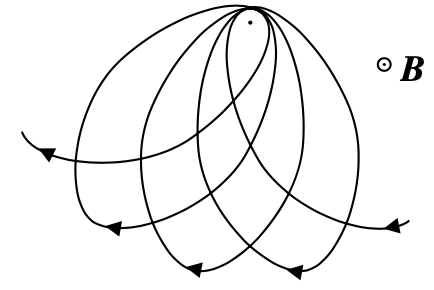
\includegraphics[width=0.2\linewidth]{../ExtFiles/larmorEffect.png}
        \caption{Larmor effect visualization.}
        \label{fig:larmorEffect}
    \end{figure}
    \begin{itemize}
        \item The picture: Suppose you have a point charge $q$ orbiting a fixed point charge $-q'$ in the presence of a constant magnetic field $\vec{B}$.
        \item Let's analyze this system to determine $q$'s trajectory.
        \item The equation of motion is
        \begin{equation*}
            m\dv[2]{\vec{r}}{t} = -\frac{k}{r^2}\hat{r}+q\dv{\vec{r}}{t}\times\vec{B}
        \end{equation*}
        where $k=qq'/4\pi\varepsilon_0$.
        \item It will be useful to move to a rotation frame. Exactly which $\vec{\omega}$ we should choose to define this rotating frame will become clear in a moment; for now, we just substitute to yield
        \begin{equation*}
            \ddot{\vec{r}}+2\vec{\omega}\times\dot{\vec{r}}+\vec{\omega}\times(\vec{\omega}\times\vec{r}) = -\frac{k}{mr^2}\hat{r}+\frac{q}{m}(\dot{\vec{r}}+\vec{\omega}\times\vec{r})\times\vec{B}
        \end{equation*}
        \item We now choose $\vec{\omega}$ to make the above computationally simpler. Indeed, choosing $\omega=-(q/2m)\vec{B}$ simplifies the above to
        \begin{equation*}
            \ddot{\vec{r}} = -\frac{k}{mr^2}\hat{r}+\left( \frac{q}{2m} \right)^2\vec{B}\times(\vec{B}\times\vec{r})
        \end{equation*}
        \item We now make an approximation: Suppose that the square of the rotation of the reference frame
        \begin{equation*}
            \omega_L^2 = \left( \frac{qB}{2m} \right)^2 \ll \frac{k}{mr^3} = \frac{qq'}{4\pi\varepsilon_0mr^3} \approx \omega_0^2
        \end{equation*}
        where $\omega_0$ is the angular velocity of $q$ in its orbit around $q'$.
        \begin{itemize}
            \item The notation $\omega_L$ will be explained shortly.
        \end{itemize}
        \item Then in this case, we can neglect the $\vec{B}\times(\vec{B}\times\vec{r})$ term to yield
        \begin{equation*}
            \ddot{\vec{r}} = -\frac{k}{mr^2}\hat{r}
        \end{equation*}
        \item Thus, in the rotating frame, the orbits are ellipses.
        \item In the inertial frame, the ellipse precesses about the direction of $\vec{B}$ with angular frequency equal to the \textbf{Larmor frequency}.
    \end{itemize}
    \item \textbf{Larmor frequency}: The angular frequency at which an elliptical orbit precesses about an applied magnetic field. \emph{Denoted by} $\bm{\omega_L}$. \emph{Given by}
    \begin{equation*}
        \omega_L = \frac{qB}{2m}
    \end{equation*}
    \item Precession of $\vec{J}$ when $\vec{B}\not\perp\vec{J}$.
    \begin{figure}[h!]
        \centering
        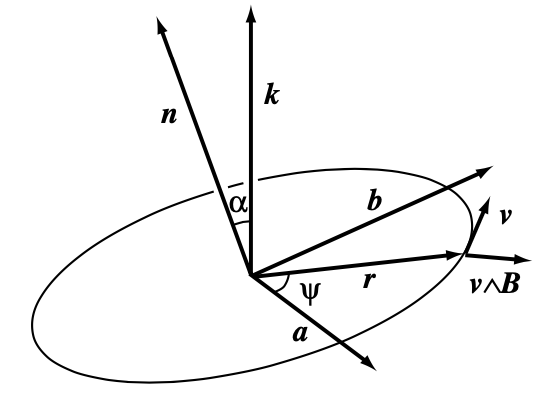
\includegraphics[width=0.35\linewidth]{../ExtFiles/Jprecession.png}
        \caption{Precession of $\vec{J}$.}
        \label{fig:Jprecession}
    \end{figure}
    \begin{itemize}
        \item The picture: A small force is exerted upon a rotating system much like the one discussed above. The small force is that of a weak magnetic field. The rotating system comprises $q$ circularly orbiting $q'$, which is fixed at the origin.
        \begin{itemize}
            \item $\khat$ defines an axis for an inertial reference frame.
            \item To define a local, rotating reference frame for the rotating system, let\dots
            \begin{itemize}
                \item $\hat{n}$ be normal to the plane of the orbit, pointing in the same direction as $\vec{J}$;
                \item $\hat{a}$ point in the direction of $\khat\times\hat{n}$;
                \item $\hat{b}$ point in the direction of $\hat{n}\times\hat{a}$.
            \end{itemize}
            \item We also take $\alpha$ to be the angle between $\khat$ and $\hat{n}$, and $\psi$ to be the angle between $\hat{a}$ and $q$'s position vector $\vec{r}$.
            \item Thus, if we fix the location of $q'$ to be the origin, then at a given moment the particle is\dots
            \begin{itemize}
                \item At position $\vec{r}=(r\cos\psi,r\sin\psi,0)$;
                \item At velocity $\vec{v}=(-v\sin\psi,v\cos\psi,0)$.
            \end{itemize}
            \item The weak, constant magnetic field is taken to be $\vec{B}=B\khat=(0,B\sin\alpha,B\cos\alpha)$.
        \end{itemize}
        \item We want to\dots
        \begin{enumerate}
            \item Prove that $\vec{J}$ precesses about $\vec{k}$ without changing magnitude;
            \item Find this precession's angular frequency.
        \end{enumerate}
        \item Thus, we will investigate $\dv*{\vec{J}}{t}$.
        \item To begin, we may write that
        \begin{equation*}
            \dv{\vec{J}}{t} = \vec{r}\times\vec{F}
            = q\vec{r}\times(\vec{v}\times\vec{B})
            = q[(\vec{r}\cdot\vec{B})\vec{v}-(\vec{r}\cdot\vec{v})\vec{B}]
        \end{equation*}
        \item Since $\vec{r}\cdot\vec{v}=0$ in a circular orbit and we have the above definitions of $\vec{r},\vec{B},\vec{v}$ in terms of the local, rotating reference frame, we may expand the above to
        \begin{align*}
            \dv{\vec{J}}{t} &= q(\vec{r}\cdot\vec{B})\vec{v}\\
            &= qBr\sin\alpha\sin\psi\vec{v}\\
            &= qBrv\sin\alpha(-\sin^2\psi,\sin\psi\cos\psi,0)
        \end{align*}
        \item We now make an approximation: Since $\vec{B}$ is weak, $\vec{J}$ will not change much in the time it takes for $q$ to make one complete orbit of $q'$. Thus, we don't care that much about the exact change in $\vec{J}$ at every position $\psi$ within that orbit; we care much more about the net change over the whole orbit. Thus, let's replace the oscillating term $(-\sin^2\psi,\sin\psi\cos\psi,0)$ with its expected value $(-1/2,0,0)$. This changes the above into
        \begin{equation*}
            \dv{\vec{J}}{t} = qBrv\sin\alpha\left( -\frac{1}{2},0,0 \right)
            = -\frac{1}{2}qBrv\sin(\alpha)\hat{a}
        \end{equation*}
        \item We have now accomplished our first task: The above shows that $\vec{J}$ moves exclusively in a direction perpendicular to it, so its magnitude remains unchanged. Moreover, this direction will cause it to precess about $\vec{k}$, as expected.
        \item We now wrap up the second task.
        \item If $\vec{J}$ is precessing about $\vec{k}$, then it's very analogous to the case surrounding Figure \ref{fig:Vrotation}. In particular, we should be able to write the above equation in the form
        \begin{equation*}
            \dv{\vec{J}}{t} = \vec{\omega}\times\vec{J}
            = \omega\khat\times\vec{J}
        \end{equation*}
        for some $\omega$.
        \item We may then solve for $\omega$ as follows, accomplishing our second task.
        \begin{align*}
            \omega\khat\times\vec{J} &= -\frac{1}{2}qBrv\sin(\alpha)\hat{a}\\
            \omega mrv\khat\times\hat{n} &= -\frac{1}{2}qBrv\sin(\alpha)\hat{a}\\
            \omega mrv\sin(\alpha)\hat{a} &= -\frac{1}{2}qBrv\sin(\alpha)\hat{a}\\
            \omega m &= -\frac{1}{2}qB\\
            \omega &= -\frac{qB}{2m}
        \end{align*}
    \end{itemize}
\end{itemize}



\section{Midterm Exam Review}
\begin{itemize}
    \item \marginnote{10/27:}Our guiding problem: Given $\vec{r}_1(0),\dots,\vec{r}_N(0)$ and $\vec{v}_1(0),\dots,\vec{v}_N(0)$, predict $\vec{r}_1(t),\dots,\vec{r}_N(t)$.
    \item So far, we've discussed only the case of 1 particle feeling an external force $\vec{F}(\vec{r},\dot{\vec{r}},t)$ due to all others.
    \item How do we determine particle motion?
    \begin{enumerate}
        \item Find \textbf{equations of motion}.
        \begin{itemize}
            \item These are second-order ODEs of the form $\ddot{\vec{r}}(t)=g(\vec{r},\dot{\vec{r}},t)$; one such ODE per particle in the system.
        \end{itemize}
        \item Solve for $r(t)$.
        \begin{itemize}
            \item $r(t)$ is the \textbf{trajectory} specified by the two initial conditions given per component.
        \end{itemize}
    \end{enumerate}
    \item In physics, the laws of classical mechanics give us the EOMs. There are two formulations of them, however.
    \begin{enumerate}
        \item Newtonian.
        \begin{itemize}
            \item The sole EOM is
            \begin{equation*}
                m\ddot{\vec{r}}(t) = \vec{F}(\vec{r},\dot{\vec{r}},t)
            \end{equation*}
        \end{itemize}
        \item Lagrangian.
        \begin{itemize}
            \item Start with the \textbf{Lagrangian}
            \begin{equation*}
                L = T-V = \frac{1}{2}m\dot{\vec{r}}^2-V(\vec{r})
            \end{equation*}
            of the system.
            \item Theorem: Trajectories are stationary points of the \textbf{action}
            \begin{equation*}
                S = \int_{t_0}^{t_1}L(q_i,\dot{q}_i)\dd{t}
            \end{equation*}
            \item This gives us equations of motion via
            \begin{equation*}
                \dv{t}\pdv{L}{\dot{q}_i} = \pdv{L}{q_i}
            \end{equation*}
            for $i=1,2,3$.
        \end{itemize}
    \end{enumerate}
    \item We now look at some important cases of this general program.
    \item Concepts from Chapter 2: Linear motion.
    \begin{enumerate}
        \item In 1D, a force is \textbf{conservative} if it depends only on position.
        \begin{itemize}
            \item Then we can find a potential energy function $V(x)=-\int_{x_0}^xF(x')\dd{x'}$ (note also that $F(x)=-\dv*{V}{x}$). From here, we can obtain the total energy $E=m\dot{x}^2/2+V(x)$, which is conserved (i.e., $E=\text{constant}$, $\dv*{E}{t}=0$).
            \item A plot of the potential $V(x)$ vs. $x$ gives lots of qualitative info on the trajectory.
        \end{itemize}
        \item Every potential energy function near a minimum (equilibrium) can be approximated as a harmonic oscillator potential.
        \begin{itemize}
            \item Taking $V(x)$ with minimum at $x^*$, let $\var{x}=x-x^*$. Then
            \begin{equation*}
                V(x) = V(x^*)+\eval{\dv{V}{x}}_{x^*}\var{x}+\frac{1}{2}\eval{\dv[2]{V}{x}}_{x^*}\var{x}^2+\cdots
            \end{equation*}
            \item Choose $V(x^*)=0$, and note that since we are at a minimum, the second term above (the slope at the minimum) equals zero.
            \item Thus,
            \begin{equation*}
                V(x^*+\var{x}) = \frac{1}{2}k\var{x}^2
            \end{equation*}
            where $k=\eval{\dv*[2]{V}{x}}_{x^*}$.
        \end{itemize}
        \item Motion in a harmonic oscillator potential.
        \begin{itemize}
            \item Our Newtonian EOM is
            \begin{equation*}
                \ddot{x}+\frac{k}{m}x = 0
            \end{equation*}
            \item This means that the system oscillates with frequency $\omega=\sqrt{k/m}$ and follows the trajectory
            \begin{equation*}
                x(t) = a\cos(\omega t-\phi)
            \end{equation*}
            where $a,\phi$ follow from the initial conditions.
            \item Damped case.
            \begin{itemize}
                \item Our Newtonian EOM is
                \begin{equation*}
                    \ddot{x}+2\gamma\dot{x}+\omega_0^2x = 0
                \end{equation*}
                where $\gamma=\lambda/2m$ and $\omega_0=\sqrt{k/m}$.
                \item In the \textbf{overdamped} case, $\gamma>\omega_0$, and the trajectory looks like Figure \ref{fig:dampedOscillatora} and has the form
                \begin{equation*}
                    x(t) = \frac{1}{2}A\e[-\gamma_+t]+\frac{1}{2}B\e[-\gamma_-t]
                \end{equation*}
                where
                \begin{equation*}
                    \gamma_\pm = \gamma\pm\sqrt{\gamma^2-\omega_0^2}
                \end{equation*}
                \item In the \textbf{underdamped} case, $\gamma<\omega_0$, and the trajectory looks like Figure \ref{fig:dampedOscillatorb} and has the form
                \begin{equation*}
                    x(t) = a\e[-\gamma t]\cos(\omega t-\theta)
                \end{equation*}
                where
                \begin{equation*}
                    \omega = \sqrt{\omega_0^2-\gamma^2} \neq \omega_0
                \end{equation*}
                \item In the \textbf{critically damped} case, $\gamma=\omega_0$, and the trajectory looks like Figure \ref{fig:dampedOscillatorc} and has the form
                \begin{equation*}
                    x(t) = (a+bt)\e[-\gamma t]
                \end{equation*}
            \end{itemize}
            \item Forced, damped case.
            \begin{itemize}
                \item Our Newtonian EOM is
                \begin{equation*}
                    \ddot{x}+2\gamma\dot{x}+\omega_0^2x = F_1\cos\omega_1t
                \end{equation*}
                \item The corresponding trajectory has the form
                \begin{equation*}
                    x(t) = a_1\cos(\omega_1t-\theta_1)+\underbrace{\text{damped solution}}_\text{transient}
                \end{equation*}
                where
                \begin{align*}
                    a_1 &= \frac{F_1/m}{\sqrt{(\omega_0^2-\omega_1^2)^2+4\gamma^2\omega_1^2}}&
                    \theta_1 &= \tan^{-1}\left( \frac{2\gamma\omega_1}{\omega_0^2-\omega_1^2} \right)
                \end{align*}
                \item For small damping, $a_1$ is a sharply peaked function of $\omega_0-\omega_1$ (see Figure \ref{fig:resa}); this is the \textbf{resonance} condition.
            \end{itemize}
        \end{itemize}
    \end{enumerate}
    \item Concepts from Chapter 3 of \textcite{bib:KibbleBerkshire}, Chapter 7 of \textcite{bib:ThorntonMarion}. Essentially, this covers 3D particle motion: Energy, angular momentum, and the Lagrangian.
    \begin{enumerate}
        \item In 3D, conservative forces satisfy
        \begin{equation*}
            \vec{\nabla}\times\vec{F} = 0
        \end{equation*}
        \begin{itemize}
            \item From here, we can derive that $V(\vec{r})$ such that $\vec{F}=-\vec{\nabla}V(\vec{r})$.
        \end{itemize}
        \item Torque, angular momentum, and central forces satisfy, respectively,
        \begin{align*}
            \vec{G} &= \vec{r}\times\vec{F}&
            \vec{J} &= \vec{r}\times\vec{p}&
            \vec{F} &= F\hat{r}
        \end{align*}
        \begin{itemize}
            \item Note:
            \begin{equation*}
                \dv{\vec{J}}{t} = \vec{G}
            \end{equation*}
            \item Central forces conserve angular momentum, i.e., $\dv*{\vec{J}}{t}=0$.
        \end{itemize}
        \item The Lagrangian in 3D.
        \begin{itemize}
            \item Lagrange's EOM generalizes to his equations of motion,
            \begin{equation*}
                \dv{t}\pdv{L}{\dot{q}_i} = \pdv{L}{q_i}
            \end{equation*}
            for $i=1,2,3$.
            \begin{itemize}
                \item Recall that $\pdv*{L}{\dot{q}_i}$ is the \textbf{generalized momentum}, and $\pdv{L}{q_i}$ is the \textbf{generalized force}.
            \end{itemize}
            \item Constraints can also be incorporated via Lagrange undetermined multipliers. Here, the equations of motion are
            \begin{align*}
                \dv{t}\pdv{L}{\dot{q}_i} &= \pdv{L}{q_i}+\sum_{j=1}^n\lambda_j(t)\pdv{f_j}{q_i}&
                f_j(q_i,t) &= 0
            \end{align*}
            for $i=1,2,3$, $j=1,\dots,n$.
            \begin{itemize}
                \item Recall that $\sum_{j=1}^n\lambda_j(t)\pdv*{f_j}{q_i}$ is the \textbf{generalized force of constraint}.
            \end{itemize}
        \end{itemize}
    \end{enumerate}
    \item Concepts from Chapter 4: Central, conservative forces.
    \begin{enumerate}
        \item A central, conservative force has the form $\vec{F}=-\hat{r}\dv*{V(r)}{r}$.
        \begin{itemize}
            \item \textbf{Central}: $\hat{r}$ direction.
            \item \textbf{Conservative}: Radial dependence only.
        \end{itemize}
        \item In this constrained scenario, motion is confined to a plane under certain conservation laws.
        \begin{itemize}
            \item The plane of motion is that which is perpendicular to $\hat{J}$, which is directionally and magnitude-wise fixed.
            \item The conservation laws are
            \begin{align*}
                \frac{1}{2}m(\dot{r}^2+r^2\dot{\theta}^2)+V(r) &= E&
                mr^2\dot{\theta} &= J
            \end{align*}
            \item Combining these, we obtain the \textbf{radial energy equation}
            \begin{equation*}
                \frac{1}{2}m\dot{r}^2+\frac{J^2}{2mr^2}+V(r) = E
            \end{equation*}
            \item From the above equation, we define the \textbf{effective potential energy}
            \begin{equation*}
                U(r) = \frac{J^2}{2mr^2}+V(r)
            \end{equation*}
            \begin{itemize}
                \item This allows us to treat the system just like a 1D potential from chapter 2 in the radial coordinate.
            \end{itemize}
            \item We can also derive the \textbf{orbit equation}
            \begin{equation*}
                \frac{J^2}{2m}\left( \pdv{u}{\theta} \right)^2+\frac{J^2}{2m}u^2+V(u) = E
            \end{equation*}
            \begin{itemize}
                \item $u=1/r$.
                \item This equation has no time $t$ in it or in any derivatives!
                \item Because of the lack of time, it relates the shape of the path $u(\theta)$ to the force law.
            \end{itemize}
        \end{itemize}
        \item For inverse square law forces, the orbits are
        \begin{align*}
            r[e\cos(\theta-\theta_0)-1] &= \ell&
            r[e\cos(\theta-\theta_0)+1] &= \ell
        \end{align*}
        \begin{itemize}
            \item The left equation corresponds to the \textbf{repulsive} case, in which $k>0$.
            \item The right equation corresponds to the \textbf{attractive} case, in which $k<0$.
            \item $\ell=J^2/m|k|$.
            \item $e=0$ gives you a circle.
            \item $e<1$ gives you an ellipse.
            \item $e=1$ gives you a parabola.
            \item $e>1$ gives you a hyperbola.
        \end{itemize}
        \item Scattering experiments can probe force laws because the force law dictates an angular dependence of particle detection via
        \begin{equation*}
            \dv{\sigma}{\Omega} = \frac{b}{\sin\theta}\left| \dv{b}{\theta} \right|
        \end{equation*}
        \begin{itemize}
            \item $b(\theta)$ can be found from $V(r)$.
        \end{itemize}
    \end{enumerate}
    \item Concepts from Chapter 5: Rotating reference frames.
    \begin{enumerate}
        \item For $\vec{b}=b_x\ihat+b_y\jhat+b_z\khat$ in the rotating frame,
        \begin{equation*}
            \left( \dv{\vec{b}}{t} \right)_\text{inertial} = \dot{\vec{b}}_\text{rotating}+\vec{\omega}\times\vec{b}
        \end{equation*}
        \item The equations of motion as measured in the \emph{rotating} frame are
        \begin{equation*}
            m\ddot{\vec{r}} = \underbrace{m\dv[2]{\vec{r}}{t}}_\text{inertial}-\underbrace{2m\vec{\omega}\times\dot{\vec{r}}\vphantom{\dv[2]{\vec{r}}{t}}}_\text{Coriolis}-\underbrace{m\vec{\omega}\times(\vec{\omega}\times\vec{r})\vphantom{\dv[2]{\vec{r}}{t}}}_\text{centrifugal}
        \end{equation*}
    \end{enumerate}
\end{itemize}




\end{document}